\documentclass[12pt, a4paper]{article}

\usepackage[utf8]{inputenc}

% Limit the page margin to only 1 inch.
\usepackage[margin=1in]{geometry}

%Imports biblatex package
\usepackage[
backend=biber,
style=alphabetic
]{biblatex}
\addbibresource{../math-342w.bib}

% Enables the `align' environment.
\usepackage{amsmath}
\usepackage{bm}
\usepackage{array}

% Provides useful environments, such as:
% - \begin{proof} ...\end{proof}
\usepackage{amsthm}
\newtheorem{proposition}{Proposition}
\theoremstyle{definition}
\newtheorem*{definition}{Definition}
\newtheorem{theorem}{Theorem}
\newtheorem{corollary}{Corollary}
\newtheorem*{example}{Example}
\newtheorem*{algorithm}{Algorithm}

% Enables using \mathbb{}, for example \mathbb{N} for the set of natural numbers.
\usepackage{amssymb}

% Allows using letters in enumerate list environment. Use, for example:
%\begin{enumerate}[label=(\alph*)]
% ...
%\end{enumerate}
\usepackage[inline]{enumitem}

% Enable importing external graphic files and provides useful commands, like \graphicspath{}
\usepackage{graphicx}
% Images are located in a directory called "images" in the current directory.
\graphicspath{{./images/}}

% Make links look better by default.
% See: https://tex.stackexchange.com/questions/823/remove-ugly-borders-around-clickable-cross-references-and-hyperlinks
\usepackage[hidelinks]{hyperref}
\usepackage{xcolor}
\hypersetup{
	colorlinks,
	linkcolor={red!50!black},
	citecolor={blue!50!black},
	urlcolor={blue!80!black}
}

% Code Listings. Source:
% https://stackoverflow.com/questions/3175105/inserting-code-in-this-latex-document-with-indentation
\usepackage{listings}
\usepackage{color}
\usepackage[most]{tcolorbox}

\definecolor{dkgreen}{rgb}{0,0.6,0}
\definecolor{gray}{rgb}{0.5,0.5,0.5}
\definecolor{mauve}{rgb}{0.58,0,0.82}

\lstset{frame=tb,
	language=Java,
	aboveskip=3mm,
	belowskip=3mm,
	showstringspaces=false,
	columns=flexible,
	basicstyle={\small\ttfamily},
	numbers=none,
	numberstyle=\tiny\color{gray},
	keywordstyle=\color{blue},
	commentstyle=\color{dkgreen},
	stringstyle=\color{mauve},
	breaklines=true,
	breakatwhitespace=true,
	tabsize=3
}

\newcommand{\prob}{\text{P}}
%\newcommand{\complement}{\mathsf{c}}
\newcommand{\test}{\text{test}}
\newcommand{\train}{\text{train}}
\newcommand{\select}{\text{select}}
\newcommand{\Dtest}{\mathbb{D}_{\test}}
\newcommand{\Dtrain}{\mathbb{D}_{\train}}
\newcommand{\Dselect}{\mathbb{D}_{\select}}
\title{Lecture 15: MATH 342W: Introduction to Data Science and Machine Learning}
\author{Sergio E. Garcia Tapia\thanks{Based on lectures of Dr. Adam Kapelner at Queens College.
See also the \href{https://github.com/kapelner/QC_MATH_342W_Spring_2025}{course GitHub page}.}}
\date{April 1st, 2025 (last updated \today)}

\begin{document}
	\maketitle
	\section*{Introduction to Model Selection}
	Last lecture, we introduced the notion of \textit{transformed} or \textit{derived}
	features. Throughout our study, we have used $p$ to denote the number of features.
	To account for features before and after transformations, we use $p_{\text{raw}}$
	to denote the number of features before transformations, and $p$ to denote
	the number of features after transformations, which includes the raw features
	and the derived features. Our motivation was to reduce misspecification
	error by allowing for a more comprehensive set $\mathcal{H}$ of candidate functions
	(for example, to fit parabolas when lines are insufficient).
	
	The problem we now face is that there are too many ways to derive features
	(with interactions, without interactions, etc). Moreover, there are too many choices
	of models, each consisting of an algorithm and a set of candidate functions.
	How can we select the best model?
	
	Suppose for now that there are $M$ pre-specified algorithm-candidate set pairs:
	\begin{align*}
		(\mathcal{A}_1, \mathcal{H}_1), (\mathcal{A}_2,\mathcal{H}_2),\ldots,
		(\mathcal{A}_M, \mathcal{H}_M)
	\end{align*}
	For example, we might have:
	\begin{align*}
		\mathcal{A}_1 &= \text{OLS},\quad \mathcal{H}_1 = \{\, w_0+w_1x \mid \bm{w}\in\mathbb{R}^2 \,\}\\
		\mathcal{A}_2 &= \text{OLS},\quad \mathcal{H}_2 = \{\, w_0+w_1x+w_2x^2\mid \bm{w}\in\mathbb{R}^3\}\\
		\mathcal{A}_3 &= \text{OLS},\quad \mathcal{H}_3 = \{\, w_0+w_1x+w_2\ln(x) \mid \bm{w}\in\mathbb{R}^3\}\\
		\mathcal{A}_4 &= \text{OLS or logistic},\quad \mathcal{H}_4 = \{\ldots\}
	\end{align*}
	We wish to:
	\begin{enumerate}[label=(\roman*)]
		\item select the best among the $M$ candidates;
		\item compute a conservative estimate of future performance for the chosen candidate;
		\item output a prediction function $g_{\text{final}}$.
	\end{enumerate}
	\begin{tcolorbox}[breakable]
		\begin{example}
			Model selection is a fundamental problem of science. For example,
			there were originally a few classical models of gravitation:
			\begin{enumerate}[label=(\arabic*)]
				\item $F = G\frac{m_1m_2}{r^2}$
				\item $F = G_1\frac{m_1m_2}{r^2} + G_2\frac{m_1m_2}{r^3}$
				\item $F = G_1\frac{m_1m_2}{r^2}e^{-G_2r}$
			\end{enumerate}
			Model (2) might have been a better fit, but there may have been
			other trade-offs that caused it losing favor over (1).
		\end{example}
	\end{tcolorbox}
	\section*{No Cross-Validation (CV)}
	Previously, we started with our set of historical data $\mathbb{D}$
	\begin{align*}
		\underbrace{
		\begin{bmatrix}
			{} & {} & {}\\
			{} & \mathbb{D} & {}\\
			{} & {} & {}
		\end{bmatrix}
		}_{n\times p}
	\end{align*}
	Then, we split (partitioned) it into $\mathbb{D}_{\text{train}}$ and $\mathbb{D}_{\text{test}}$:
	\begin{align*}
		&\underbrace{
		\begin{bmatrix}
			{} & \mathbb{D}_{\text{train}} & {}\\
			{} & {} & {}
		\end{bmatrix}
		}_{n_{\text{train}}\times p}\quad
		\underbrace{
		\begin{bmatrix}
			{} & \mathbb{D}_{\text{test}} & {}
		\end{bmatrix}
		}_{n_{\text{test}}\times p},\quad n_{\train} + n_{\test} = n
	\end{align*}
	We did this to obtain honest estimate of out-of-sample performance.
	A natural extension of this idea is to run each of the $M$ algorithms on $\Dtrain$
	with their respective candidate sets, and compute the out-of-sample performance metric of
	each on $\Dtest$:
	\begin{align*}
		g_1&=\mathcal{A}_1(\mathbb{D}_{\text{train}}, \mathcal{H}_{1})\implies
		\text{predict on }\Dtest\implies
		\bm{e}_{\test,1}\implies oosRMSE_1\\
		g_2&=\mathcal{A}_2(\mathbb{D}_{\text{train}}, \mathcal{H}_{2})\implies
		\text{predict on }\Dtest\implies
		\bm{e}_{\test,2}\implies oosRMSE_2\\
		&\vdots\\
		g_M&=\mathcal{A}_M(\mathbb{D}_{\text{train}}, \mathcal{H}_{M})\implies
		\text{predict on }\Dtest\implies
		\bm{e}_{\test,M}\implies oosRMSE_M\\
	\end{align*}
	Then, we can pick the algorithm-candidate set pair for which the out-of-sample
	RMSE metric is minimized:
	\begin{align*}
		m_* = \underset{m\in \{1,2,\ldots,M\}}{\text{argmin}}\{oosRMSE_m\}
	\end{align*}
	Hence, according to this scheme, the best model is $(\mathcal{A}_{m_*}, \mathcal{H}_{m_*})$.
	In expectation (that is, on average), this is a good way to choose the best
	model. However, what we do not get out of this is an estimate of future
	predictive performance. If $M$ is large, it's possible that we ``get lucky",
	meaning we get an algorithm-candidate set pair that optimizes for $\Dtrain$ and $\Dtest$.
	That is, we may get a pair $(\mathcal{A}_k, \mathcal{H}_k)$ that ``accidentally"
	does well on $\Dtrain$ and $\Dtest$, but still performs poorly out-of-sample.
	This is a form of overfitting. We need to be careful to treat $\Dtest$ as an
	opaque box that we open only once.
	
	To address this, we further partition $\mathbb{D}$ so that we have three
	pieces:
	\begin{align*}
		\underbrace{
			\begin{bmatrix}
				{} & \mathbb{D}_{\text{train}} & {}\\
			\end{bmatrix}
		}_{n_{\text{train}}\times p}\quad
		\underbrace{
			\begin{bmatrix}
				{} & \mathbb{D}_{\text{select}} & {}
			\end{bmatrix}
		}_{n_{\text{select}}\times p}\quad
		\underbrace{
			\begin{bmatrix}
				{} & \mathbb{D}_{\text{test}} & {}
			\end{bmatrix}
		}_{n_{\text{test}}\times p}
	\end{align*}
	where $n=n_\train + n_\select + n_\test$ is the total number of observations and
	\begin{align*}
		n_\test &= \frac{1}{K_\test}\cdot n = \text{Number of rows in }\Dtest\\
		n-n_\train&=\left(1- \frac{1}{K_\test}\right)\cdot n = \text{Number of rows in }\Dtrain\cup \Dselect = \mathbb{D} \setminus \Dtest\\
		n_\select &= \frac{1}{K_\select}(n-n_\train) = \frac{1}{K_\select}\left(1 - \frac{1}{K_\test}\right)n=\text{Number of rows in }\Dselect
	\end{align*}
	Then we repeat the process from earlier, replacing $\Dtest$ with $\Dselect$:
	\begin{itemize}
		\item \textbf{Step 1}: Train all $M$ models on $\Dtrain$ and compute their respective
		out-of-sample metrics on $\Dselect$:
		\begin{align*}
			g_1&=\mathcal{A}_1(\mathbb{D}_{\text{train}}, \mathcal{H}_{1})\implies
			\text{predict on }\Dselect\implies
			\bm{e}_{\select,1}\implies oosRMSE_1\\
			g_2&=\mathcal{A}_2(\mathbb{D}_{\text{train}}, \mathcal{H}_{2})\implies
			\text{predict on }\Dselect\implies
			\bm{e}_{\select,2}\implies oosRMSE_2\\
			&\vdots\\
			g_M&=\mathcal{A}_M(\mathbb{D}_{\text{train}}, \mathcal{H}_{M})\implies
			\text{predict on }\Dselect\implies
			\bm{e}_{\select,M}\implies oosRMSE_M\\
		\end{align*}
		\item \textbf{Step 2}: Select the algorithm and candidate set
		$(\mathcal{A}_{m*}, \mathcal{H}_{m_*})$ for which the out-of-sample metric
		was the smallest:
		\begin{align*}
			m_* = \underset{m\in \{1,2,\ldots,M\}}{\text{argmin}}\{oosRMSE_m\}
		\end{align*}
		\item \textbf{Step 3}: Run $\mathcal{A}_{m_*}$, but now on $\Dtrain\cup \Dselect$
		to obtain a new prediction function:
		\begin{align*}
			g_{m_{**}} = \mathcal{A}_{m_*}(\Dtrain \cup \Dselect, \mathcal{H}_{m_*})
		\end{align*}
		(in class we overloaded the $g_{m*}$ name, but here I will use double-star to distinguish
		$g_{m_{**}}$ obtained by running $\mathcal{A}_{m_*}$ on $\Dtrain\cup\Dselect$
		from $g_{m_*}$ which was obtained by running $\mathcal{A}_{m_*}$ only on $\Dtrain$).
		\item \textbf{Step 4}: Compute the out-of-sample metric for $g_{m_{**}}$ by predicting on $\Dtest$:
		\begin{align*}
			g_{m_{**}}\implies \text{predict on } \Dtest\implies \bm{e_{m_{**}}}\implies oosRMSE_{m_{**}}
		\end{align*}
		\item \textbf{Step 5}: We run algorithm $m_{*}$ now on the entire data set:
		\begin{align*}
			g_{\text{final}} = \mathcal{A}_{m_*}\left(
			\underbrace{\Dtrain \cup \Dselect \cup \Dtest}_{\mathbb{D}}, \mathcal{H}_{m_*}
			\right)
		\end{align*}
		The value of $oosRMSE_{m_{**}}$ computed in the previous step is now a conservative
		estimate of the future performance of $g_{\text{final}}$.
	\end{itemize}
	We refer to this algorithm as \textbf{No Cross-Validation (No CV)}.
	We might view this as a meta-algorithm, where each algorithm $\mathcal{A}_m$ is viewed
	as a feature. If $M$ is too large, we are at risk of overfitting.
	\section*{Select Cross-Validation (CV)}
	In the No-CV approach, each of $\Dtrain$, $\Dselect$, and $\Dtest$ was fixed.
	We can improve upon that approach by fixing $\Dtest$, but applying a $K_\select$-fold
	cross-validation on each of the $M$ models.
	\begin{itemize}
		\item \textbf{Step 1}: Fix a value for $K_\test$, denoting the proportion
		of $\mathbb{D}$ to use for $\Dtest$, so that $\Dtest$ is fixed for the rest
		of the algorithm, which will be used in the final validation step.
		Hence, $\mathbb{D}\setminus \Dtest$ is also fixed.
		\item \textbf{Step 2}: Fix a value of $K_\select$, denoting the proportion $\mathbb{D}\setminus \Dtest$
		that will be used for testing each of the $M$ algorithms. Note that $K_\select$
		is fixed but $\Dselect$ is not.
		\item \textbf{Step 3}: Shuffle the data set $\mathbb{D}\setminus \Dtest$.
		\item \textbf{Step 4}: For $m\in \{1,2,\ldots,M\}$, that is, for each pair
		$(\mathcal{A}_m,\mathcal{H}_m)$:
		\begin{itemize}
			\item For $k\in \{1,2,\ldots,K_\select\}$:
			\begin{itemize}
				\item Take the next piece (the $k$th piece) of proportion $K_\select$
				from $\mathbb{D}\setminus \Dtest$ to use as $\mathbb{D}_{\text{select}, k}$
				(say, we start from the bottom of $\mathbb{D}\setminus \Dtest$).
				What remains is $\mathbb{D}_{\text{train}, k}$.
				\item Compute a prediction function $g_{k}^{(m)}=\mathcal{A}_m(\mathbb{D}_{\train, k}, \mathcal{H}_m)$.
				\item Predict on $\mathbb{D}_{\select, k}$ using $g_{k}^{(m)}$, yielding error
				vector $\bm{e}_k^{(m)}$.
			\end{itemize}
			\item After doing $K_\select$ folds for the $m$th model, stack the residual
			vectors into a vector of length $n_\train + n_\select$:
			\begin{align*}
				\bm{e}_m = 
					\begin{bmatrix}
						\bm{e}_{K\select}^{(m)}\\
						\vdots\\
						\bm{e}_{2}^{(m)}\\
						\bm{e}_{1}^{(m)}
					\end{bmatrix}
			\end{align*}
			\item Compute $oosRMSE_m$ using $\bm{e}_m$. (How? Is it the mean?)
		\end{itemize}
		\item \textbf{Step 5}: Now we have $oosRMSE_1,oosRMSE_2,\ldots,oosRMSE_M$. Take $m_*$ to be
		\begin{align*}
			m_* = \underset{m\in\{1,2,\ldots,M\}}{\text{argmin}}
			\{
			oosRMSE_m
			\}
		\end{align*}
		\item \textbf{Step 6}: Train model $(\mathcal{A}_{m_*}, \mathcal{H}_{m_*})$
		on $\mathbb{D}\setminus \Dtest$ to get
		$g_* = \mathcal{A}_{m_*}(\mathbb{D}\setminus \Dtest, \mathcal{H}_{m_*})$.
		\item \textbf{Step 7}: Predict using $g_{*}$ on $\Dtest$ to obtain
		$oosRMSE_*$.
		\item \textbf{Step 8}: Train model $(\mathcal{A}_{m_*}, \mathcal{H}_{m_*})$
		on $\mathbb{D}$ to get $g_{\text{final}} = \mathcal{A}_{m_*} (\mathbb{D}, \mathcal{H}_{m_*})$. We use $oosRMSE_{*}$ as a conservative estimate of the
		future out-of-sample performance of $g_{\text{final}}$.
	\end{itemize}
	There is a trade-off here in that this requires more computation, but we may get
	a better model.
	\section*{Select and Test CV}
	A third approach we can use is called \textbf{select and test CV}, or
	\textbf{nested resampling}. This approach reduces the variation of $oosRMSE_*$
	in $g_{\text{final}}$ by varying $\Dtest$ rather than keeping it fixed.
	We pay in computational expense, which is determined by $K_\test\cdot K_\select\cdot M$.
	However, we are more sure that we pick the best of our $M$ models.
	Note the algorithm for select-CV had a nested loop; this algorithm would
	add yet another level of nesting $K_\test$.
	
	\href{
		https://mlr.mlr-org.com/articles/tutorial/nested_resampling.html}{Click here to navigate to a page with an example to visualize nested resampling}.
	\section*{Applying Model Selection Procedures}
	The three model selection procedures we just discussed (no CV, select CV, and
	select and test CV) are useful in many settings. The three we will study are:
	\begin{enumerate}[label=(\arabic*)]
		\item Pick one model among $M$ pre-specified modeling precedures, provide
		a conservative estimate of future performance, and compute $g_{\text{final}}$.
		\item Greedy Forward Stepwise Modeling.
		\item Hyperparameter Selection.
	\end{enumerate}
	Recall that there are infinitely-many candidate sets. Therefore (1) can be unrealistic.
	(2) provides an alternative.
	\section*{Greedy Forward Stepwise Modeling}
	\begin{itemize}
		\item \textbf{Step 0}: Create a very large set of derived features so
		that $\mathcal{H}$ can be very expansive (large). For example:
		\begin{align*}
			\{
			&x_1,\ldots,x_p, x_1^2,\ldots,x_p^2,x_1^3,\ldots,x_p^3,\ln(x_1),\ldots,\ln(x_p)\\
			&x_1x_2,\ldots,x_1x_p,\ldots,x_2x_3,\ldots,x_2x_p,\ldots,x_{p-1}x_p\\
			&x_1x_2x_3,\ldots,x_{p-2}x_{p-1}x_{p},\sin(x_1),\ldots,\sin(x_p)
			\}
		\end{align*}
		Note that $(p+1)\gg n$. We could build a design matrix $X$ that tracks these
		features, but it would not be invertible, and hence we would not be able to
		apply OLS. How many OLS models do we have with such a large set? A total of
		$2^{p+1}$! We will search this space greedily (not optimally), which will
		give us a decent solution.
		
		Begin with some $g_0\in\mathcal{H}_0$ (e.g. the null model), where
		$\mathcal{H}_0=\{w_0:w_0\in \mathbb{R}\}$ (this is our ``seed").
		\item \textbf{Step 1}: For each of the $p$ features, fit OLS to
		\begin{align*}
			\mathcal{H} = \{\,
			w_0+w_1\underbrace{()}_{\text{feature}}\mid \bm{w}\in\mathbb{R}^2
			\,\}
		\end{align*}
		using $\Dtrain$. Then predict using $\Dselect$ to obtain an $oosRMSE$ for each.
		Record the best feature $j_*$ based on the best $oosRMSE$.
		\item \textbf{Step 2}: For each of the remaining $p-1$ features, fit OLS to
		\begin{align*}
			\mathcal{H} = \{\,
			w_0 + w_1(\text{feature}_{j_{*_1}}) + w_2\underbrace{()}_{\text{feature}} \mid
			\bm{w}\in\mathbb{R}^3
			\,\}
		\end{align*}
		using $\Dtrain$. Then predict using $\mathbb{D}_\select$ to compute an $oosRMSE$ for
		each. Record the best feature $j_{*_2}$ based on the best $oosRMSE$.
		Note that it cannot be $j_{*_1}$ because that feature is not under consideration
		in the remaining $p-1$ features.
		\item \textbf{Step F}: After $F$ steps, where $F$ is a pre-determined maximum, or
		at each step, look at the results of the $oosRMSE$ from $\Dselect$, and when you
		are sure that the $oosRMSE$ is increasing, stop. The reason it may start to
		increase is due to overfitting. Suppose this occurs at iteration $t_*$
		(see Figure~\ref{fig:greedy-stepwise-oosRMSE}).
		\begin{figure}
			\centering
			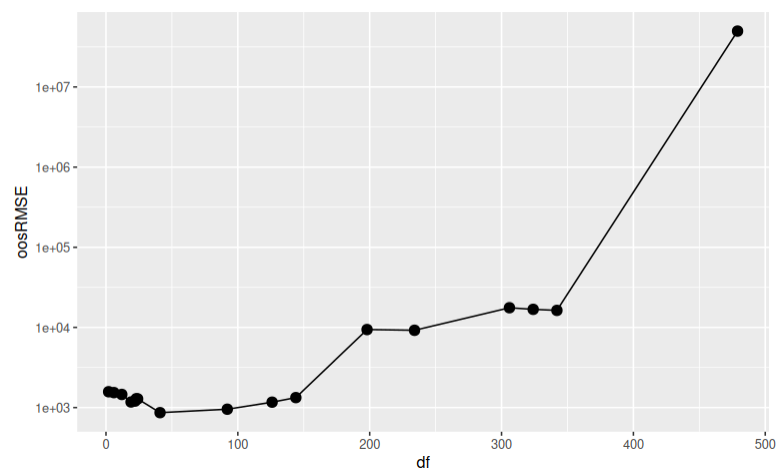
\includegraphics[width=0.8\textwidth]{greedy-forward-stepwise-oosRMSE-by-iteration}
			\caption{Greedy Forward Stepwise Modeling, tracking the out-of-sample RMSE
			across iterations}
			\label{fig:greedy-stepwise-oosRMSE}
		\end{figure}
		Then compute a model
		\begin{align*}
			g_* = \mathcal{A}(\Dtrain \cup \Dselect, \mathcal{H}_{t_*})
		\end{align*}
		Use $g_*$ to predict on $\Dtest$ to get $\bm{e}$ and compute $oosRMSE$, an
		estimate of future performance. Then output
		\begin{align*}
			g_{\text{final}} = \mathcal{A}(\mathbb{D}, \mathcal{H}_{t_*})
		\end{align*}
	\end{itemize}
	\section*{Hyperparameter Selection}
	Recall the SVM algorithm with the Vapnik objective function:
	\begin{align*}
		\mathcal{A}_{\lambda}:\bm{b} = \underset{\bm{w}\in\mathbb{R}^{p+1}}{\text{argmin}}
		\left\{
		\frac{1}{n}\sum_{i=1}^{n}H_i + 
		\lambda \|\bm{w}\|
		\right\}
	\end{align*}
	As before, $\|\bm{w}\|$ is the size of the wedge, which we are trying
	to maximize. For each $i$, $H_i$ denotes the $i$th hinge error, which is $0$
	for the points that are correctly classified and otherwise it is a positive
	number denoting the distance of a misclassified point from the hyperplane across
	the wedge defined by the hyperplane. The value $\lambda$ is the hyperparameter
	of the algorithm, which needs to be specified numerically in advance. Hence,
	each different value of $\lambda$ results in a different algorithm because
	the objective function changes, so that we have a family of algorithms
	$\{\mathcal{A}_\lambda\}_{\lambda\in\mathbb{R}}$.
	
	Suppose we create a grid of $M$ values that $\lambda$ can take on. For example:
	\begin{align*}
		\lambda_{\text{grid}} = \{
			10^{-3}, 10^{-2}, 10^{-1}, 10^0, 10^{1}, 10^{2}
		\}
	\end{align*}
	Now we can use no-CV, select-CV, or nested resampling to pick the best
	$\lambda\in \lambda_{\text{grid}}$. The weakness in this approach is having
	to pre-specify $M$ models, which in this setting translates in pre-specifying
	$M$ hyperparameters. To do this effectively, we need a reasonable range of $\lambda$
	values to consider. If our algorithm has more than one hyperparameter,
	our $\lambda_{\text{grid}}$ might be two-dimensional, i.e., a set of tuples.
	\pagebreak
	\printbibliography
\end{document}